\documentclass[border=4pt]{standalone}
\usepackage[T1]{fontenc}
\usepackage[utf8]{inputenc}
\usepackage{lmodern}
\usepackage{tikz}
\usetikzlibrary{positioning,arrows.meta}
\begin{document}
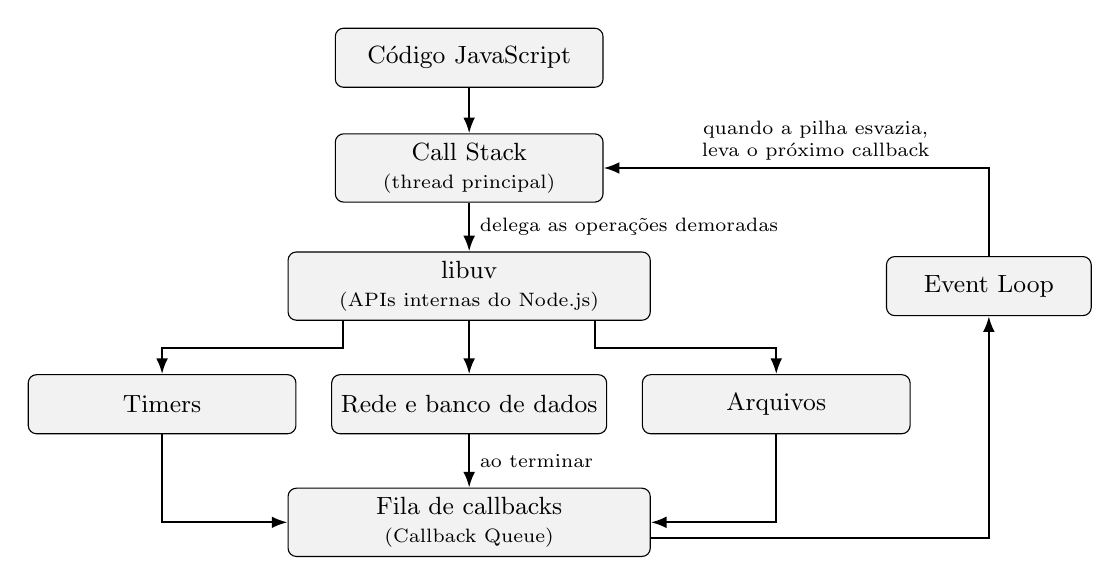
\begin{tikzpicture}[
  caixa/.style={draw, rounded corners=3pt, fill=black!5, minimum width=3.4cm,
                minimum height=0.75cm, align=center, font=\small},
  seta/.style={-{Latex[length=2mm]}, thick},
  rotulo/.style={font=\scriptsize, fill=white, inner sep=1.5pt}
]
  \node[caixa] (codigo) at (0,0) {Código JavaScript};
  \node[caixa] (pilha)  at (0,-1.4) {Call Stack\\[-1pt]{\scriptsize (thread principal)}};
  \node[caixa, minimum width=4.6cm] (libuv) at (0,-2.9) {libuv\\[-1pt]{\scriptsize (APIs internas do Node.js)}};
  \node[caixa] (timer)   at (-3.9,-4.4) {Timers};
  \node[caixa] (rede)    at (0,-4.4) {Rede e banco de dados};
  \node[caixa] (arquivo) at (3.9,-4.4) {Arquivos};
  \node[caixa, minimum width=4.6cm] (fila) at (0,-5.9) {Fila de callbacks\\[-1pt]{\scriptsize (Callback Queue)}};
  \node[caixa, minimum width=2.6cm] (loop) at (6.6,-2.9) {Event Loop};

  \draw[seta] (codigo) -- (pilha);
  \draw[seta] (pilha) -- node[rotulo, right=2pt] {delega as operações demoradas} (libuv);
  \draw[seta] (libuv.south) -- (rede.north);
  \draw[seta] (libuv.south) ++(-1.6,0) |- ++(0,-0.35) -| (timer.north);
  \draw[seta] (libuv.south) ++(1.6,0) |- ++(0,-0.35) -| (arquivo.north);
  \draw[seta] (timer.south) |- (fila.west);
  \draw[seta] (rede.south) -- node[rotulo, right=2pt] {ao terminar} (fila.north);
  \draw[seta] (arquivo.south) |- (fila.east);
  \draw[seta] (fila.east) ++(0,-0.2) -| (loop.south);
  \draw[seta] (loop.north) |- (pilha.east);
  \node[rotulo, align=center, above=1pt] at (4.4,-1.4) {quando a pilha esvazia,\\leva o próximo callback};
\end{tikzpicture}
\end{document}
